\documentclass[11pt, a4paper]{article}\usepackage[]{graphicx}\usepackage[]{xcolor}
% maxwidth is the original width if it is less than linewidth
% otherwise use linewidth (to make sure the graphics do not exceed the margin)
\makeatletter
\def\maxwidth{ %
  \ifdim\Gin@nat@width>\linewidth
    \linewidth
  \else
    \Gin@nat@width
  \fi
}
\makeatother

\definecolor{fgcolor}{rgb}{0.345, 0.345, 0.345}
\newcommand{\hlnum}[1]{\textcolor[rgb]{0.686,0.059,0.569}{#1}}%
\newcommand{\hlsng}[1]{\textcolor[rgb]{0.192,0.494,0.8}{#1}}%
\newcommand{\hlcom}[1]{\textcolor[rgb]{0.678,0.584,0.686}{\textit{#1}}}%
\newcommand{\hlopt}[1]{\textcolor[rgb]{0,0,0}{#1}}%
\newcommand{\hldef}[1]{\textcolor[rgb]{0.345,0.345,0.345}{#1}}%
\newcommand{\hlkwa}[1]{\textcolor[rgb]{0.161,0.373,0.58}{\textbf{#1}}}%
\newcommand{\hlkwb}[1]{\textcolor[rgb]{0.69,0.353,0.396}{#1}}%
\newcommand{\hlkwc}[1]{\textcolor[rgb]{0.333,0.667,0.333}{#1}}%
\newcommand{\hlkwd}[1]{\textcolor[rgb]{0.737,0.353,0.396}{\textbf{#1}}}%
\let\hlipl\hlkwb

\usepackage{framed}
\makeatletter
\newenvironment{kframe}{%
 \def\at@end@of@kframe{}%
 \ifinner\ifhmode%
  \def\at@end@of@kframe{\end{minipage}}%
  \begin{minipage}{\columnwidth}%
 \fi\fi%
 \def\FrameCommand##1{\hskip\@totalleftmargin \hskip-\fboxsep
 \colorbox{shadecolor}{##1}\hskip-\fboxsep
     % There is no \\@totalrightmargin, so:
     \hskip-\linewidth \hskip-\@totalleftmargin \hskip\columnwidth}%
 \MakeFramed {\advance\hsize-\width
   \@totalleftmargin\z@ \linewidth\hsize
   \@setminipage}}%
 {\par\unskip\endMakeFramed%
 \at@end@of@kframe}
\makeatother

\definecolor{shadecolor}{rgb}{.97, .97, .97}
\definecolor{messagecolor}{rgb}{0, 0, 0}
\definecolor{warningcolor}{rgb}{1, 0, 1}
\definecolor{errorcolor}{rgb}{1, 0, 0}
\newenvironment{knitrout}{}{} % an empty environment to be redefined in TeX

\usepackage{alltt}

\usepackage[top=1 in, bottom = 1 in, left = 1 in, right = 1 in ]{geometry}

\usepackage{amsmath, amssymb, amsfonts}
\usepackage{enumerate}
\usepackage{array}
\usepackage{multirow}
\usepackage{dingbat}
\usepackage{fontawesome5}
\usepackage{tasks}
\usepackage{bbding}
\usepackage{xcolor}

\definecolor{col1}{HTML}{e75e05}
\definecolor{stack_red}{HTML}{DB4437}
\definecolor{stack_yellow}{HTML}{F4B400}
\definecolor{stack_cyan}{HTML}{08e2f0}
\definecolor{stack_blue}{HTML}{4285F4}
\definecolor{stack_green}{HTML}{0F9D58}

\title{MSMS - 105}
\author{Ananda Biswas}
\date{}
\IfFileExists{upquote.sty}{\usepackage{upquote}}{}
\begin{document}

\maketitle

\begin{center}
\textbf{Assignment 02}
\end{center}


\OrnamentDiamondSolid \hspace{0.5cm} \textcolor{blue}{\textbf{Objective :}} To design and develop an animated plot that visually represents the progress of loading. \\

\faArrowAltCircleRight[regular] \textcolor{col1}{\textbf{\textit{Idea}}} : We try to animate a ball falling from top and it gets bigger as it falls. The balls get stacked in 10 layers each with 10 balls representing a total of 100 percent. \textcolor{stack_red}{\textbf{RED}}, \textcolor{stack_yellow}{\textbf{YELLOW}}, \textcolor{stack_cyan}{\textbf{CYAN}}, \textcolor{stack_blue}{\textbf{BLUE}}, \textcolor{stack_green}{\textbf{GREEN}} layers respectively denote \textcolor{stack_red}{\textbf{20}}, \textcolor{stack_yellow}{\textbf{40}}, \textcolor{stack_cyan}{\textbf{60}}, \textcolor{stack_blue}{\textbf{80}}, \textcolor{stack_green}{\textbf{100}} percentage of total loading done. \\


\faArrowAltCircleRight[regular] \textcolor{col1}{\textbf{\textit{Implementation}}} : 

\begin{knitrout}
\definecolor{shadecolor}{rgb}{0.969, 0.969, 0.969}\color{fgcolor}\begin{kframe}
\begin{alltt}
\hldef{pause} \hlkwb{<-} \hlkwa{function}\hldef{(}\hlkwc{seconds}\hldef{) \{}
  \hldef{start} \hlkwb{<-} \hlkwd{Sys.time}\hldef{()}
  \hlkwa{while}\hldef{((}\hlkwd{Sys.time}\hldef{()} \hlopt{-} \hldef{start)} \hlopt{<} \hldef{seconds) \{\}}
\hldef{\}}
\end{alltt}
\end{kframe}
\end{knitrout}

\begin{knitrout}
\definecolor{shadecolor}{rgb}{0.969, 0.969, 0.969}\color{fgcolor}\begin{kframe}
\begin{alltt}
\hlkwd{par}\hldef{(}\hlkwc{bg} \hldef{=} \hlsng{"black"}\hldef{)}
\hlkwd{plot}\hldef{(}\hlnum{NA}\hldef{,} \hlnum{NA}\hldef{,}
     \hlkwc{xlim} \hldef{=} \hlkwd{c}\hldef{(}\hlnum{1}\hldef{,} \hlnum{10}\hldef{),}
     \hlkwc{ylim} \hldef{=} \hlkwd{c}\hldef{(}\hlnum{1}\hldef{,} \hlnum{10}\hldef{),}
     \hlkwc{xaxt} \hldef{=} \hlsng{"n"}\hldef{,}
     \hlkwc{yaxt} \hldef{=} \hlsng{"n"}\hldef{,}
     \hlkwc{xlab} \hldef{=} \hlsng{""}\hldef{,}
     \hlkwc{ylab} \hldef{=} \hlsng{""}\hldef{)}
\end{alltt}
\end{kframe}
\end{knitrout}

\begin{knitrout}
\definecolor{shadecolor}{rgb}{0.969, 0.969, 0.969}\color{fgcolor}\begin{kframe}
\begin{alltt}
\hldef{ball_colors} \hlkwb{<-} \hlkwd{rep}\hldef{(}\hlkwd{c}\hldef{(}\hlsng{"#DB4437"}\hldef{,} \hlsng{"#F4B400"}\hldef{,} \hlsng{"#08e2f0"}\hldef{,} \hlsng{"#4285F4"}\hldef{,} \hlsng{"#0F9D58"}\hldef{),}
                   \hlkwd{rep}\hldef{(}\hlnum{2}\hldef{,} \hlnum{5}\hldef{))}
\end{alltt}
\end{kframe}
\end{knitrout}

\begin{knitrout}
\definecolor{shadecolor}{rgb}{0.969, 0.969, 0.969}\color{fgcolor}\begin{kframe}
\begin{alltt}
\hlkwa{for} \hldef{(t} \hlkwa{in} \hlnum{1}\hlopt{:}\hlnum{10}\hldef{) \{}
  \hldef{pop} \hlkwb{<-} \hlnum{1}\hlopt{:}\hlnum{10}

  \hlkwa{for}\hldef{(k} \hlkwa{in} \hlnum{1}\hlopt{:}\hlnum{10}\hldef{)\{}

    \hlkwa{if}\hldef{(k} \hlopt{<} \hlnum{10}\hldef{)\{}
      \hldef{num} \hlkwb{<-} \hlkwd{sample}\hldef{(pop,} \hlnum{1}\hldef{)}
    \hldef{\}} \hlkwa{else}\hldef{\{}
      \hldef{num} \hlkwb{<-} \hldef{pop[}\hlnum{1}\hldef{]}
    \hldef{\}}

    \hldef{cl} \hlkwb{<-} \hlkwd{rep}\hldef{(}\hlsng{"black"}\hldef{,} \hlnum{10}\hlopt{-}\hldef{t}\hlopt{+}\hlnum{1}\hldef{)}

    \hlkwa{for} \hldef{(m} \hlkwa{in} \hlnum{1}\hlopt{:}\hldef{(}\hlnum{10}\hlopt{-}\hldef{t}\hlopt{+}\hlnum{1}\hldef{)) \{}
      \hldef{cl[m]} \hlkwb{<-} \hldef{ball_colors[t]}
      \hlkwa{if}\hldef{(t} \hlopt{!=} \hlnum{10}\hldef{)\{}
        \hlkwd{points}\hldef{(}\hlkwc{x} \hldef{=} \hlkwd{rep}\hldef{(num,} \hlkwd{length}\hldef{(}\hlnum{10}\hlopt{:}\hldef{t)),}
               \hlkwc{y} \hldef{=} \hlnum{10}\hlopt{:}\hldef{t,}
               \hlkwc{col} \hldef{= cl,}
               \hlkwc{pch} \hldef{=} \hlnum{19}\hldef{,}
               \hlkwc{cex} \hldef{=} \hlkwd{seq}\hldef{(}\hlnum{1}\hldef{,} \hlnum{4}\hldef{,} \hlkwc{length} \hldef{=} \hlnum{10}\hlopt{-}\hldef{t}\hlopt{+}\hlnum{1}\hldef{))}
      \hldef{\}} \hlkwa{else}\hldef{\{}
        \hlkwd{points}\hldef{(}\hlkwc{x} \hldef{= num,} \hlkwc{y} \hldef{=} \hlnum{10}\hldef{,} \hlkwc{col} \hldef{= cl,} \hlkwc{pch} \hldef{=} \hlnum{19}\hldef{,} \hlkwc{cex} \hldef{=} \hlnum{4}\hldef{)}
      \hldef{\}}
      \hlkwd{pause}\hldef{(}\hlnum{0.15}\hldef{)}
      \hldef{cl} \hlkwb{<-} \hlkwd{rep}\hldef{(}\hlsng{"black"}\hldef{,} \hlnum{10}\hlopt{-}\hldef{t}\hlopt{+}\hlnum{1}\hldef{)}
    \hldef{\}}

    \hldef{index} \hlkwb{<-} \hlkwd{which}\hldef{(pop} \hlopt{==} \hldef{num)}
    \hldef{pop} \hlkwb{<-} \hldef{pop[}\hlopt{-}\hldef{index]}
  \hldef{\}}
\hldef{\}}
\end{alltt}
\end{kframe}
\end{knitrout}

\faArrowAltCircleRight[regular] \textcolor{col1}{\textbf{\textit{Stages of the Animation}}} : 

\begin{table}[!htbp]

\begin{center}
\begin{tabular}{ccc}

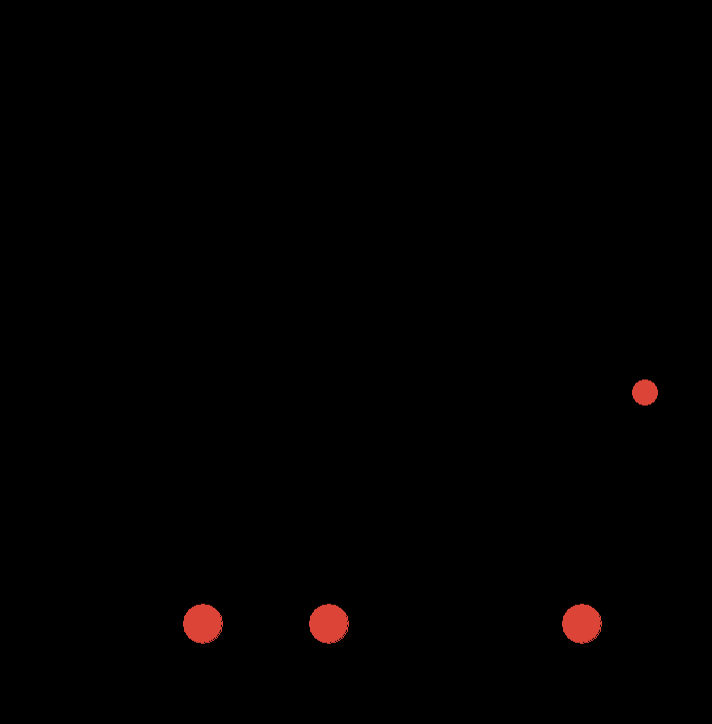
\includegraphics[scale = 0.35]{3} & 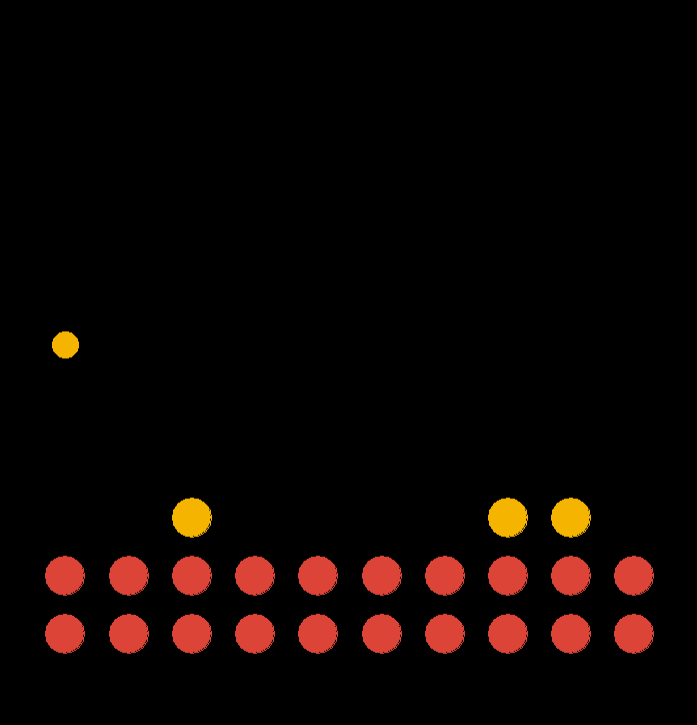
\includegraphics[scale = 0.35]{20} & 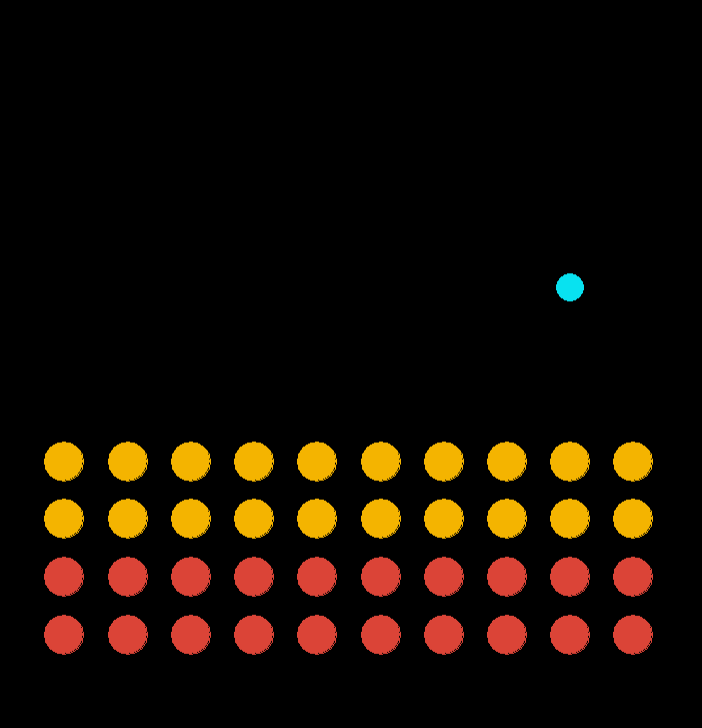
\includegraphics[scale = 0.35]{40} \\

3 \% done and in-progress & 20 \% done and in-progress & 40 \% done and in-progress \\

& & \\

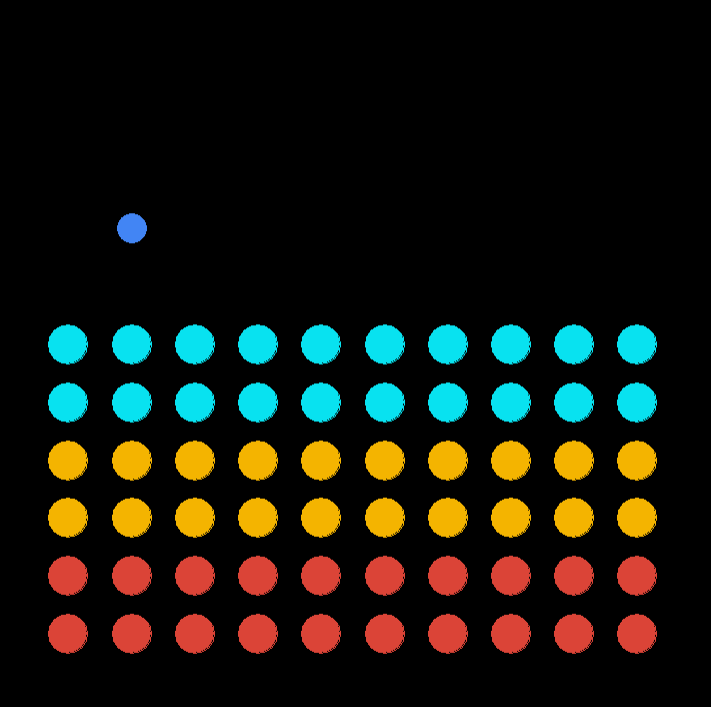
\includegraphics[scale = 0.35]{60} & 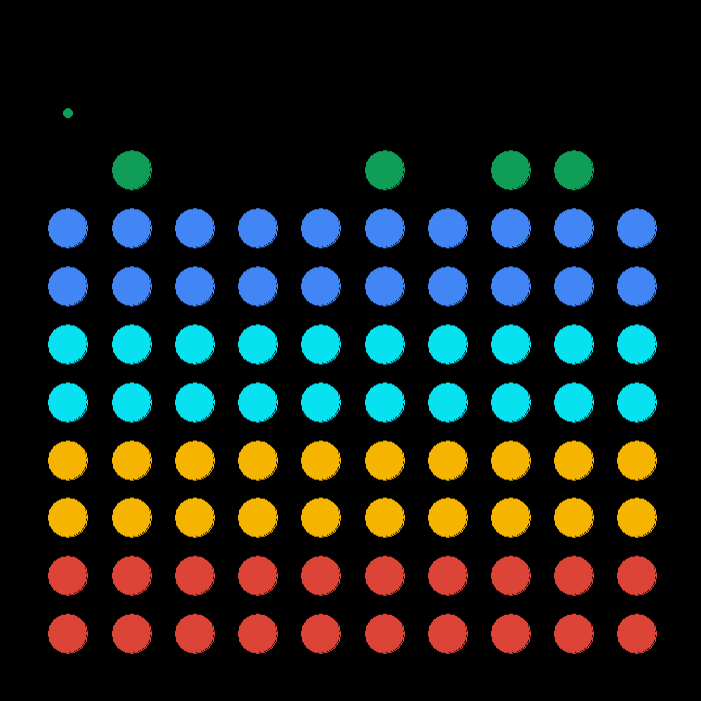
\includegraphics[scale = 0.35]{80} & 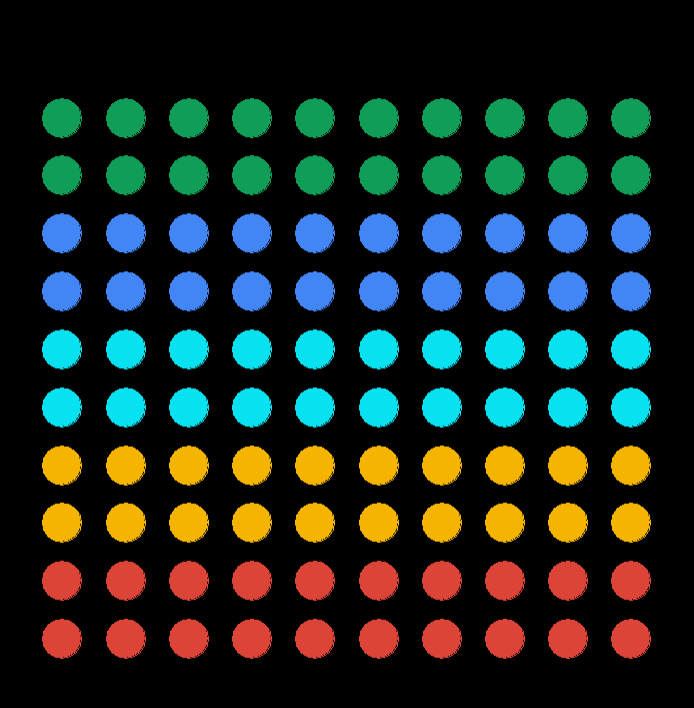
\includegraphics[scale = 0.35]{100} \\

60 \% done and in-progress & 80 \% done and in-progress & 100 \% done \\


\end{tabular}
\end{center}
\end{table}

\end{document}
